\chapter{Selected algorithms for graphs represented in RDF}
\label{chap:theoretical-attachment}

In this chapter, we will describe and analyze two algorithms that we implemented when developing the D3.js Chord Visualizer (Section~\ref{sec:visualizers:chord}). This particular \emph{visualizer} is using a chord diagram to visualize relationships and their strengths among entities. As we explained in Section~\ref{sec:visualizers:chord:rgml}, the chord diagram is actually visualizing a directed multi graph (as understood in the graph theory). As the input, it takes an adjacency matrix of this graph (or more specifically, of a subgraph that the user selected for visualization), which is what our first algorithm is responsible for. The second algorithm is responsible for generating a random sample subgraph which can be then shown to the user.

As we wanted both our algorithms to work even for potentially very large graphs, loading them into memory and representing them in native data structures was not an option. Because of this requirement, we needed to work directly with the RDF representation of the graph which presented a certain challenge.

\section{Calculating the graph adjacency matrix for the chord diagram}

In our first implementation (when we needed quick results) we would simply load the whole graph into memory, represent it using native data structures and then work with this representation. This approach proved itself sufficient and actually pretty efficient for small graphs (for example the asylum seekers data set, see Subsection \ref{sec:visualizers:chord:data-sets} for data sets description). Compared to SPARQL queries (which involve accessing the hard drive or even communication over network in case the triple store is on a separate machine), in-memory operations are way faster and fetching couple of hundreds nodes and edges in every request was bearable (we needed just two queries to fetch the nodes and the edges).

The situation changed (the performance dropped) when we started experimenting with the air routes data set, containing around 8000 airports and almost 70000 routes. To improve performance and support even bigger graphs, we decided to re-implement the service so that the complexity of any operation would depend on the size of the input, not on the size of the graph. That typically means, that we would never do operations like loading all nodes or edges into memory. Obviously, we can guarantee this assumption only in our own code. The triple store (e. g. Virtuoso) might work differently.

\subsection{Adjacency matrix}

Let us have a look at how generating the adjacency matrix for the chord diagram works. An adjacency matrix for a directed graph is a square matrix where the $(i, j)$ value indicates whether there is an edge going from the node $i$ to the node $j$. Typically this value is either $1$ (nodes are connected in this direction) or $0$ (nodes are not connected in this direction). In our case, however, the graph is a directed weighted multigraph. Such a graph is impossible to represent using this kind of adjacency matrix because we would need to distinguish somehow between having two nodes connected by $10$ edges of weight $1$ or by $1$ edge of weight $10$.  But as we have explained in Section \ref{sec:visualizers:chord:rgml}, these two situations are considered equal which is given by the characteristics of the chord visualization. The \emph{visualizer} performs a simple aggregation which sums the weights of all multi-edges. Therefore the $(i,j)$ value actually corresponds to the sum of weights of all edges going from $i$ to $j$.

\subsection{Problem description}

The input of our function is a list of nodes (more specifically their URIs) of size $n$, for which we want to generate the adjacency matrix (remember that we are generating the adjacency matrix for a subgraph that the user selected for visualization). Let us denote the number of all nodes in the graph by $N$ and the number of all edges in the graph by $M$. Let us denote the maximum number of edges between two nodes by $c$. That means that $M$ is $O(cN^2)$ and that we can perform the aggregation mentioned above in $O(c)$ for any two nodes.

How much is $c$?  The situation is the simplest with the asylum seekers data set. One edge using its weight represents the number of asylum applicants between two countries in a particular month. The data set contains data for only one year, there is $12$ months to a year, and that is $c$. That means that $c$ is a constant and we can leave it out from the complexities. The situation gets more complicated with the other two data sets. As of the air routes data set, one edge corresponds to one air route between two cities. We can assume that $c$ in this case will not be very high, which is given firstly by the limited size of both airports and also by the limited demand of people wanting to travel between two cities. Unfortunately, we are not able to make any more accurate assumptions. Similarly to the contracts data set, where one edge corresponds to a contract between two companies. Therefore we will include $c$ in all complexities but the reader should keep in mind what this number is and that it typically will not grow out of proportions.

Our adjacency matrix has $n^2$ values. The \emph{straightforward} algorithm would be to make a SPARQL query for every two nodes $(i, j)$ to fetch the edges going from $i$ to $j$ and calculate the aggregated weight. The overall complexity would be $O(cn^2)$ which is as fast as it can be (it is simply not possible to generate a square matrix of size $n$ faster than $O(n^2)$  and the aggregation is $O(c)$). The problem here is that we make $O(n^2)$ SPARQL queries and as we have already explained, a SPARQL query is by far slower than any in-memory operation. So our primary target became to reduce the number of SPARQL queries.

\subsection{Algorithm description}

Let us write down the final algorithm that we ended up with:

\begin{enumerate}
\item For each node, fetch all its incident edges (both outgoing and incoming). Put all fetched edges in a single data structure and remove duplicates.
\item Put all nodes in a Scala \texttt{Set} which is a data structure with $O(1)$  \emph{MEMBER} operation.
\item Create an empty adjacency matrix.
\item Iterate over the fetched edges and if an edge connects two nodes that are both in our \texttt{Set}, update the corresponding value in the adjacent matrix.
\item Return the matrix.
\end{enumerate}

The important improvement is that even though we fetch more edges than we need (some of them we do not need at all, some of them are fetched twice), suddenly we perform only $O(n)$ SPARQL queries (for each node we need two queries, one for outgoing edges, one for incoming) which means a huge performance boost. According to our experiments, this approach is more than 4 times faster in the air routes data set than the very first one which involved fetching the whole graph. Note that we did not conduct any exact reproducible benchmarking, we simply measured the times of HTTP requests on the client which gave us the improvement from around $7$ seconds to around $1.5$ second (and that is very noticeable when working with the user interface). But what is the complexity of this algorithm?

\subsection{Analysis}

Let us denote the number of all fetched nodes by $m$. Note that it includes duplicates as well. In the first step, we first fetch the edges, which is $O(m)$, and then we remove the duplicates. That does not add any extra complexity as we can simply iterate through all edges again and use a hash table to remove duplicates. All edges are identified by unique URIs which makes this very straightforward (plus we are leveraging Scala data structures to do all this work for us anyway). The second step is $O(n)$ using the same logic and the third step, initializing the matrix, is clearly $O(n^2)$. In the fourth step we iterate over all edges, now without duplicates. That means that the actual number will be less than $m$, but let us just consider it as $O(m)$. Each iteration is done in constant time (we just access the matrix and update the value with the current edge’s weight) which gives us the overall $O(m)$ complexity for this step.

Putting this all together, we get the complexity of $O(MAX(n^2, m))$. The cardinal question now is how much is $m$. For sparse graphs where a node has typically just a few incident edges, we get close to $O(n^2)$ as $m$ is $O(n)$ (for each input node we fetch just a few edges). On the other hand, for very dense graphs (close to complete graphs) where $M \sim cN^2$, we get $m \sim ncN$ as every input node is adjacent to almost all nodes in the graph and therefore it has almost $cN$ incident edges (we must not forget to count the multi edges). And all of them are fetched.

This clearly breaks one of the assumptions that we promised to guarantee in the beginning. The complexity of this approach does depend (in some special cases) on the size of the whole graph. Specifically, this approach might get slow for very large dense graphs. The other \emph{straightforward} algorithm which is truly $O(cn^2)$ (as it makes one SPARQL query with constant size response for every potential edge between input nodes) could give better results. On the other hand, none of the graphs from our three data sets resembled a complete graph.

The truth is that it is almost impossible to decide what is the best solution as there are too many factors that a theoretical analysis cannot comprehend. For example, if the triple store was on a different machine with increased network latency, then reducing the number of SPARQL queries to minimum would become an absolute necessity. We experimented with different approaches as described in the previous paragraphs, and for those three data sets that we are working with, this last approach gave us the best results. Also our analysis shows a good potential for scalability when working with larger graphs.

One question remains to be answered though. In the first step of our algorithm, why don’t we, instead of fetching all incident edges of a particular node, fetch just those that we need, i. e., between this particular node and the rest of input nodes? We could surely generate such a SPARQL query. We could even possibly generate a query that would return the whole subgraph induced by given input nodes. Unfortunately, our experience shows that such complicated queries, that are dynamically generated from an arbitrary number of input parameters (the input nodes) or use very often \texttt{UNIONs}, do not perform reliably well. That means that they do not finish or take significantly longer than couple of separate SPARQL queries providing the same functionality. For example, we found out that it is usually faster to use two queries to fetch edges between two nodes (one for every direction) instead of one query with a \texttt{UNION}. And that is a very simple example. Another problematic aspect is that sometimes it is necessary to use more advanced SPARQL constructs in such queries. That always creates a risk that such a feature will not be properly supported by the triple store. Therefore we chose to prefer simpler but more reliable SPARQL queries and do any complex calculations by ourselves.

\section{Sampling the graph using Forest Fire algorithm}

When the \emph{searchable} lens (see Subsection \ref{sec:visualizers:chord:fresnel}) is not available or the user has not created any named lists yet, the D3.js Chord Visualizer displays a sample visualization. It takes a random subgraph and shows it to the user. The reason behind this is that we want to give the user at least some idea of what kind of data is in the graph. The size of the sample is at this moment 30 nodes which is, as we already mentioned, roughly the number of nodes that can still be reasonably visualized using the chord diagram. Also if the whole graph is less than 30 nodes (which is not that unimaginable), then the sample visualization actually displays all there is to see and can be published as it is.

Sampling the graph, i. e., choosing the nodes for the sample visualization, turned out to be an interesting problem. Given how the chord diagram works, our main concern was that the sampling method should ideally return nodes that have at least some edges between them. If the returned sample subgraph was an independent subgraph, then the chord diagram would come out completely empty. Our second concern was at least a reasonable speed even for very large graphs as we did not want to keep the user waiting too long.

\subsection{Highest degree method}

Our first sampling approach was based on node degrees. We would sort all nodes by their degree (specifically, by the number of outgoing edges) in descendant order and then take the first 30 nodes. The idea behind this was that the nodes with highest degrees were likely to have edges between them. This idea proved correct (at least for our data sets) and we were getting pretty decent results out of it. A distinct advantage was that this sampling method was very easy to implement.

Nevertheless, it had disadvantages. Namely, the following three:

\begin{itemize}
\item There was a possibility that for certain types of graphs this approach would yield no results. For example, imagine a graph that consists of many completely independent components which have the shape of a “star”, i. e., all nodes in a component are connected only to one central node which consequently has a very high degree. The sampling method would only select those component “centers” which are,  however, completely independent. Even though we did not come across such a graph during our experiments, we think that the sampling method should be able to deal with it.
\item This method would not scale well for large graphs. Calculating degrees for all nodes in the graph is an expensive operation and it clearly depends on the graph size. We would prefer a sampling method whose speed (complexity) would solely depend on the sample size, i. e., it would perform well even on very large graphs.
\item Lastly, the generated sample does not resemble the original graph in any way. If it does, then only by accident. We will get to what \emph{resemble} means in this case later but it means that some predefined characteristics should not differ significantly between the original graph and the sampled graph.

\end{itemize}
In the future paragraphs, we will refer to this algorithm as to the \emph{highest degree} method. We should also note that the current implementation of this method does not take weights into account. Therefore it will be biased towards nodes with lots of edges and it will ignore nodes with \emph{heavy} edges. Depending on a data set, it might give undesired results.

\subsection{General algorithm requirements}

Based on the experience we gained from the \emph{highest degree} method, we were able to summarize the requirements for the sampling algorithm.

\begin{itemize}
\item \textbf{Usable output}. Given the visualization characteristics (the chord diagram), we want the algorithm to avoid independent sets, if possible, as those would yield empty visualizations.
\item \textbf{Speed}. We need the sampling algorithm to work fast even for large graphs which means that its speed should depend on the sample size rather than on the size of the original graph. \emph{Speed} is a bit vague term but in this case it cannot be simply substituted with complexity. One crucial limitation is that we cannot load the whole graph in the memory as it would immediately break the initial requirement. This means that we have to work with the original RDF representation of the graph, i.e., the sampling algorithm also needs to optimize the SPARQL queries that are used to access the graph in the triplestore. 
\item \textbf{Resemblance}. The sample graph should resemble the original graph, i.e., the visualization of the sample graph should give the user an idea of how the original graph looks like. Formally this means that certain characteristics (or metrics) of the original graph should be preserved by the sampling method. These characteristics may include 
\emph{average and standard deviation of degree}~\cite{krishnamurthy2005reducing},
\emph{degree distribution}~\cite{krishnamurthy2005reducing},
\emph{spectral analysis}~\cite{krishnamurthy2005reducing},
\emph{distance distribution}~\cite{gilbert2004compressing} or
\emph{connected component size}~\cite{rafiei2005effectively}.

\end{itemize}
\subsection{Choosing Forest Fire algorithm}

Clearly, we were not the first ones with the need to sample a large graph. This problem is pretty common, especially in the area of network topologies. A typical task is to get an idea of how a real-life network represented as a graph looks like, or to run a simulation on it. As such a network would often be very large, one would firstly need to somehow reduce it (\emph{take a sample}). Obviously, the reduction must maintain the base characteristics of the original graph for e.g. the simulation to give meaningful results.

In "Compressing Network Graphs"~\cite{gilbert2004compressing}, the authors suggest two different approaches for reducing the graph size, \emph{importance compression scheme} and \emph{similarity compression scheme}. In the first approach, the sample graph is induced by selected \emph{important} nodes. The \emph{importance} may be based on a pure topological characteristic of a node (e.g. node degree) or on some specific external information (e.g. in the case of networks, routers would be considered as important nodes). In the second approach, the graph size is reduced by contracting \emph{similar} nodes. \emph{Similar} in this case means for example that nodes share a certain number of adjacent nodes. Unfortunately, neither of those two approaches would fit our requirements. Both the \emph{importance} and the \emph{similarity} would have to be first calculated for the whole graph which clearly breaks the \textbf{speed} requirement. Note that the \emph{importance compression scheme} using node degree as the \emph{importance} metric is, as a matter of fact, our \emph{highest degree} method.

"Reducing Large Internet Topologies for Faster Simulations"~\cite{krishnamurthy2005reducing} presents several random-based sampling methods, divided into three base groups.

\begin{itemize}
\item \textbf{Deletion methods} based on randomly deleting nodes, edges or both.
\item \textbf{Contraction methods} based on contracting adjacent nodes.
\item \textbf{Exploration methods} which involve traversing through the graph either using Breadth-first search or Depth-first search.
\end{itemize}

The first two approaches are very similar: we start with the original graph and we keep reducing it until we reach the target size. Unfortunately, both these approaches are breaking our \textbf{speed} requirement as we would need to start with making a copy of the original graph. On the other hand, the exploration methods show clear potential. Firstly, we do not need to traverse through the whole graph (the \textbf{speed} requirement), secondly, given their nature they favor connected subgraphs (the \textbf{usable output} requirement).

Considering its name, the "Effectively Visualizing Large Networks Through Sampling"~\cite{rafiei2005effectively} paper was promising at first but it soon turned out that this paper is focused a bit differently. It describes an iterative method of sampling when the user can see the current selected sample visualized on a screen and by giving instructions to the software, he is enabled to \emph{grow} the sample. The sampling itself is very simple as it is based on random nodes and edges selection. The paper distinguishes \emph{global grow}, when the current sample is extended with more randomly selected nodes, and \emph{local grow}, when the current sample is extended with randomly selected nodes that are adjacent to the current sample. Clearly, none of this is useful for our purposes.

Finally, the paper  "Sampling from Large Graphs" \cite{leskovec2006sampling} presents and compares several different sampling methods organized in the following three groups.

\begin{itemize}
\item \textbf{Sampling by random node selection}. We select the nodes at random, either uniformly or with probability depending on certain node attributes.
\item \textbf{Sampling by random edge selection}. We select the edges at random. To get better results, sometimes it is necessary to combine this approach with random node selection.
\item \textbf{Sampling by exploration}. This approach involves traversing through the graph. A typical example is \emph{random walk} or the Forest Fire algorithm.
\end{itemize}

All the sampling methods are fairly algorithmically simple. The authors of \cite{leskovec2006sampling} state that there exist more advanced approaches which are however computationally expensive and therefore unsuitable for large graphs. The random approaches meet our \textbf{speed} requirements (we would be just querying random nodes or edges from the triplestore until we would reach the required sample size) but they might be more inclined to select an independent set (the \textbf{usable output} requirement). The exploration methods, as we already explained, are more reliable in this matter and the speed is also sufficient.

From all the presented algorithms, we chose the Forest Fire algorithm, which combines the exploration approach with randomness. As we will show, it meets all our requirements. It also gave the best results to the authors~of~\cite{leskovec2006sampling}. We start by describing the algorithm, then we show an actual implementation and finally we analyze the algorithm and show how it deals with the aforementioned issues. We also try to compare it with the \emph{highest degree} method as that is the only other sampling approach that we implemented.

\subsection{Algorithm description}

\cite{leskovec2006sampling} is unfortunately a bit inconsistent in defining the algorithm. They give a short overview and then in the appendix they present the following more detailed description:

\begin{displayquote}
We first choose node v uniformly at random. We then generate a random number $x$ that is geometrically distributed with mean $p_f/(1-p_f)$. Node v selects x out-links incident to nodes that were not yet visited. Let $w_1 , w_2 , \ldots, w_x$ denote the other ends of these selected links. We then apply this step recursively to each of $w_1, w_2, \ldots, w_x$ until enough nodes have been burned. As the process continues, nodes cannot be visited a second time, preventing the construction from cycling. If the fire dies, then we restart it, i.e. select new node $v$ uniformly at random. We call the parameter $p_f$ the forward burning probability.
\end{displayquote}

The core idea is clear but the overview and the description differ in several aspects. Besides, the authors also refer to another paper "Graphs over Time: Densification Laws, Shrinking Diameters and Possible Explanations" \cite{leskovec2005graphs} which is where this algorithm was originally defined. In this paper, it was used for modeling graph evolution (so instead of reducing graphs it was responsible for generating graphs). The algorithm as described in \cite{leskovec2005graphs} uses binomial distribution and defines two different probabilities of \emph{burning}, one for outgoing nodes and one for incoming.

In our implementation, we decided to go with the binomial distribution as it is easily simulated with simple \emph{coin flipping}. As a matter of fact, this sampling method is nothing else but an enhanced version of Breadth-first search. We start the \emph{fire} from a randomly chosen node and then spread it over its incident edges to its surroundings. The key difference is that when traversing over an edge, we \emph{flip a coin} with certain probability ($p_f$ for outgoing edges, $p_b$ for incoming edges) to determine whether the \emph{fire} should \emph{spread} over this edge to the other node and \emph{burn} it. The algorithm runs until we collect enough nodes. If we run out of nodes to burn (we are in a small connected component), we choose another random node and start over.

Our implementation also takes weights into account. \emph{Heavier} edges have higher chance to \emph{burn}. Specifically, if an edge has the weight of 2, it counts as two edges with weight 1, i. e., we \emph{flip the coin} twice for this particular edge.

\subsection{Implementation}

As this part is fairly algorithmically interesting (considering the rest of the thesis), we decided to share here a (almost) full implementation of the algorithm. The algorithm parameters are following:

\begin{itemize}
\item \texttt{graph} -- an object representing the graph we are sampling)
\item \texttt{size} -- size of our sample
\item \texttt{useWeights} -- if weights should be taken into account as described in the previous paragraph
\item \texttt{pF} -- forward burning probability $p_f$ 
\item \texttt{pB} -- backward burning probability $p_b$
\end{itemize}

\begin{verbatim}
val graph, size, useWeights, pF, pB

/** Run the actual Forest Fire algorithm to generate the sample. */
def makeSample: Seq[String] = {
  var sample = Set.empty[String]
  while (sample.size < Math.min(size, graph.nodeCount)) {
    // Pick a random node and run BFS from it. If the fire "dies out" before burning
    // enough nodes for our sample, pick another node and run BFS again.
    val v = randomNode.uri
    if (!sample.contains(v))
      sample = burn(sample + v, Seq(v))
  }

  sample.toSeq
}

/**
  * Pick a random node. As the SPARQL support for randomness varies across different engines,
  * we decided to use a more reliable solution. We generate a random OFFSET between 0 and
  * graph node count. We return the node at this offset.
  */
def randomNode: Node = nodes(evaluation, random.nextInt(graph.nodeCount), 1).get.head

/**
  * This is the core BFS recursive function that spreads the "fire" from the current
  * {@code frontier} to the adjacent (unburnt) nodes, creating a new frontier which is
  * added to the {@code sample}. The function is then recursively called on the new frontier.
  *
  * @param sample set of nodes we have collected so far
  * @param frontier nodes at the "frontier" of the fire from where it spreads to the graph
  * @return sample with all discovered "burnt" nodes.
  */
def burn(sample: Set[String], frontier: Seq[String]): Set[String] = {
  // As traversing through the graph using SPARQL queries is rather expensive, we need to
  // avoid unnecessary queries and stop the algorithm as soon as we have enough nodes.
  if (sample.size >= size)
    return sample

  // Iterate over all burning nodes at the frontier and spread fire from each node to its
  // adjacent nodes. We have to make sure to avoid burning the same node twice.
  val nextFrontier = frontier
    .flatMap(spread)
    .filterNot(sample.contains)
    .distinct
    .take(size - sample.size) // To make sure that we don't collect more nodes than we need.

  if (nextFrontier.isEmpty)
    sample
  else
    burn(sample ++ nextFrontier, nextFrontier)
}

/**
  * Return those adjacent nodes of {@code node} that "caught on fire", i. e. the nodes
  * that should "burn" and become part of the next frontier. In standard BFS implementation,
  * this would simply return all adjacent nodes.
  */
def spread(node: String): Seq[String] = {
  incidentEdges(evaluation, node).getOrElse(Seq())
    .filter(edge => choose(edge, probability(node, edge)))
    .map(edge => theOther(node, edge))
}
\end{verbatim}

\begin{verbatim}
/** "Flip a coin" with probability {@code p} and return whether {@code edge} should burn */
def choose(edge: Edge, p: Double): Boolean = {
  // When weights are enabled, we're simulating multiple coin tosses for a single edge. One
  // "heads" is enough to get the edge burnt. To determine such probability, we use the
  // standard school trick. The probability is determined as "1 - (1 - p)^n" where {@code p}
  // is the probability of "heads" and n is number of tosses (1 or {@code useWeights} when
  // weights are enabled).
  random.nextFloat() < 1 - Math.pow(1 - p, if (useWeights) edge.weight else 1)
}

/** Determine the probability of whether {@code edge} (relatively to {@code node}) will burn */
def probability(node: String, edge: Edge): Double = {
  if (direction(node, edge) == Outgoing || !graph.directed) pF else pB
}

/** Return "the other" node of {@code edge) relatively to {@code node} */
def theOther(node: String, edge: Edge): String = {
  if (direction(node, edge) == Outgoing) edge.target else edge.source
}

/** Determine direction of {@code edge} relatively to {@code node} */
def direction(node: String, edge: Edge): EdgeDirection = {
  if (edge.source == node) Outgoing else Incoming
}
\end{verbatim}

\subsection{Analysis}

Let us now discuss the properties of this algorithm. Our first concern was that the sampling method should ideally always return something that is visualizable with the chord diagram, i. e., nodes that have some edges between them (the \textbf{usable output} requirement). The  Forest Fire algorithm is based on traversing over edges. Therefore it is very unlikely that it would return an independent set (unless, of course, there is nothing else in the graph).

The second requirement was the \textbf{speed}. Unlike the \emph{highest degree} method, Forest Fire will work even for very large (reasonable) graphs. Just as required, its complexity depends on the sample size, not on the size of the whole graph. We will only visit (\emph{burn}) as many nodes as we need for our sample. As what \emph{reasonable} means: this algorithm behaves similarly to the one we used for calculating the adjacency matrix. For every node added to our sample, we fetch all its incident edges. That is how BFS works. If the graph is close to a full graph (i. e., each node is connected to almost all other nodes in the graph), then the performance will degrade with the graph size.

We also required that the algorithm should ideally optimize the number of SPARQL queries as it presents a potential bottleneck. For example, a simple sampling method that picks nodes from the graph at random (as mentioned in \cite{rafiei2005effectively} or \cite{leskovec2006sampling}) would make one SPARQL query for each node (we admit that it is possible that some triplestore engines would allow us to select all random nodes at once). Forest Fire algorithm behaves very similarly because we have to make one SPARQL query for each expanded node to get its adjacent nodes. There is a slight difference though. Forest Fire algorithm is essentially BFS which means that the \emph{fire} spreads in iterations. In each iteration, all nodes in the current \emph{frontier} are expanded and their adjacent nodes (that \emph{caught on fire}) are added to the sample and to the next \emph{frontier}. It is clear that once we reach the target sample size, we do not have to expand the last \emph{frontier}. Hypothetically, if each iteration doubles the sample size (from each node the \emph{fire spreads} to two new nodes on average), we do not have to expand half of the nodes in the sample which means 50\% less SPARQL queries. This does not change the complexity in any way, but if the SPARQL queries are the bottleneck (e.g. the triplestore is accessed over an unreliable network), Forest Fire algorithm would  in such an extreme case work twice as fast compared to the random approach. However, in such a situation the \emph{highest degree} method would probably offer the best performance as it only queries the triple store twice (once of nodes, once for edges).

As of the actual real life performance, we experienced a significant boost over the \emph{highest degree} method, especially for the large air routes data set. Note that we did not conduct any exact reproducible benchmarking, but simply by observing the HTTP requests we measured the improvement from 3 seconds to 500 milliseconds. Such a difference is easily noticeable when working with the user interface.

Lastly, we cared about the \textbf{resemblance} between the original graph and the sample subgraph. In general, sampling is useful when the original graph is too large for standard tools. If we are able to make a sample whose characteristics are similar to the characteristics of the original graph (a \emph{realistic} sample), we can then apply the standard tools on the sample (as it is significantly smaller) and get reasonable results. To measure the deviation from the original graph, \cite{leskovec2006sampling} proposes two goals: 

\begin{itemize}
\item \textbf{Scale-down goal} which simply compares certain characteristics (e.g. degree distribution) between the sample and the original graph.
\item \textbf{Back-in-time goal} which corresponds to traveling back in time and trying to mimic the past versions of the original graph.
\end{itemize}

The paper provides exact definitions for both goals but those are not important for our cause. According to the paper, the Forest Fire gives the best results for both of  them and that is why chose it. The question is whether it actually works (specifically compared to the \emph{highest degree} method).

Another conclusion in \cite{leskovec2006sampling} is that 15\% sample is usually enough to match the defined properties of the original graph. In the air routes data set, we sample 30 out of 8000 nodes which is less than 0.4\%. It is clear that in this particular case the chance that we will get with our sample close to the original graph is practically zero. Does this mean that the Forest Fire method utterly fails in this perspective?

It certainly does not give us results \emph{similar} to the original graph as defined in \cite{leskovec2006sampling} but it definitely does give us different results than the \emph{highest degree} method. Compare the sample produced using \emph{highest degree} method (Figure \ref{fig:chord-highest-degree}) and the sample produced by Forest Fire algorithm (Figure \ref{fig:chord-forest-fire}).

\begin{figure}
	\centering
	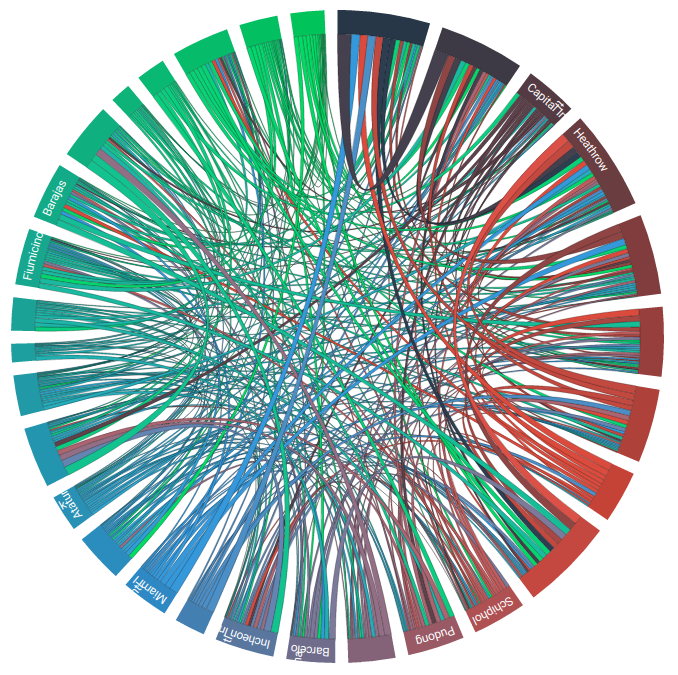
\includegraphics[width=100mm]{img/07_chord_highest_degree}
	\caption{D3.js Chord Visualizer: The air routes data set sampled with the \emph{highest degree} method. The algorithm apparently returns the 30 \emph{busiest} airports in the data set.}
    \label{fig:chord-highest-degree}
\end{figure}

\begin{figure}
	\centering
	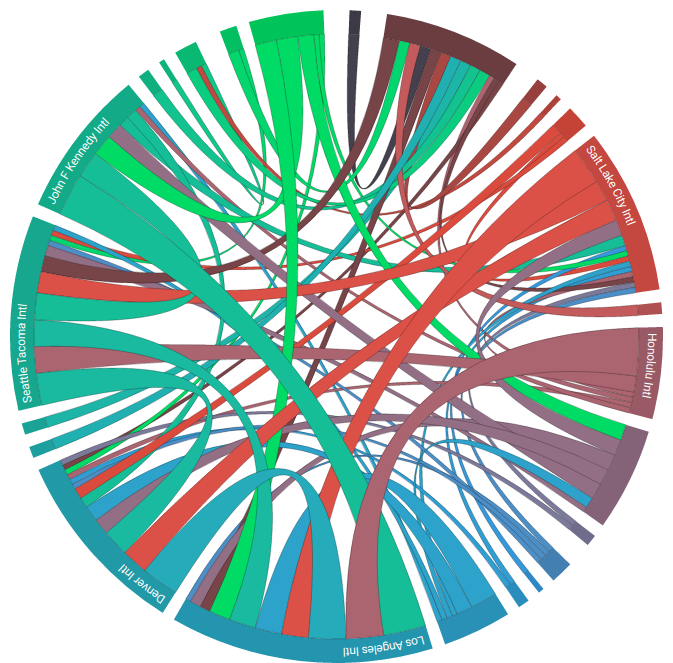
\includegraphics[width=100mm]{img/07_chord_forest_fire}
	\caption{D3.js Chord Visualizer: The air routes data set sampled with the Forest Fire method. The result is way more diverse as both small and big airports are displayed.}
    \label{fig:chord-forest-fire}
\end{figure}

We might say that whereas the \emph{highest degree} method is biased towards the most important nodes in the data set, the Forest Fire method will give the user a way more diverse result. Depending on a situation, both approaches might be useful. One of the possible improvements might be that we could let the user manually choose the sampling method as a way to explore the data set.

To sum it up, let us walk again through the three requirements and compare Forest Fire algorithm to the \emph{highest degree} method.

\begin{itemize}
\item \textbf{Usable output}. Compared to the \emph{highest degree} method, Forest Fire algorithm is less inclined to return independent sets which is thanks to the underlying BFS. Obviously, if most of the graph are independent nodes, then even Forest Fire algorithm could return an empty sample.
\item \textbf{Speed}. The complexity of Forest Fire algorithm does not depend on the graph size (except for the full graphs). That means that this algorithm will perform well even for very large graphs.
\item \textbf{Resemblance}. We explained that given the very small sample size, we cannot objectively measure the resemblance between the original graph and the sample. Nevertheless, Forest Fire algorithm does provide more diverse results.
\end{itemize}

Forest Fire algorithm clearly demonstrates its superiority and that is why we chose it as the default sampling algorithm.

There is one last remark we would like to make on this topic. The Forest Fire algorithm can be configured with the forward $p_f$ and backward $p_b$ probabilities. The forward probability is the probability of \emph{fire} \emph{spreading} over outgoing edges whereas the backward probability is the probability of \emph{fire} \emph{spreading} over incoming edges. In \cite{leskovec2006sampling} the authors try to determine the values for which they get the best results. As we already discussed, in our case it is hard to measure the resemblance between the original graph and the sample. We also mentioned that the authors of \cite{leskovec2006sampling} are a bit inconsistent in the exact algorithm description which makes it impossible to reproduce their results. Given this fact we slightly altered the algorithm: we used binomial distribution instead of geometric (as suggested in \cite{leskovec2005graphs}) because there is the nice BFS enhanced with \emph{coin flipping} analogy making the algorithm more straightforward to explain and implement. This all means that the values measured in \cite{leskovec2006sampling} are more or less irrelevant for us.

Nevertheless, this certainly does not mean that those parameters do not matter. With setting $p_f$ to $1$ (or a value close to $1$) we change the algorithm to standard BFS. So for example, if our first randomly selected node is a small American airport (from the air routes data set), the sample will contain only airports from that area. On the other hand, setting $p_f$ (and $p_b$) to $0$ turns off the search completely and we are simply selecting 30 random nodes from the data set. The sample is then completely arbitrary. We decided to leave $p_f$ to $0.2$ and $p_b$ to $0.05$ as suggested in  \cite{leskovec2006sampling}. These values produced \emph{reasonable} results and we had no reason to change them.
